\documentclass[12pt]{article}
\usepackage[a4paper, total={6in, 8in}]{geometry}
\usepackage{setspace}
\usepackage{amsmath}
\usepackage{amssymb}
\usepackage{witharrows}
\usepackage{lipsum}
\usepackage{indentfirst}
\usepackage{mathtools}
\usepackage{layout}
\usepackage{xcolor}
\usepackage{amsmath}
\usepackage{systeme}
\usepackage{blindtext}
\usepackage{sidenotes}
\usepackage{multicol}
\usepackage{fancyhdr}
\usepackage{indentfirst}
\usepackage{systeme}
\usepackage{hyperref}
\usepackage{natbib}
\usepackage{indentfirst}
\usepackage{mwe}
\usepackage{epigraph}
\usepackage[skip=10pt plus1pt]{parskip}
\WithArrowsOptions{displaystyle,tikz=blue}

\begin{document}
\pagenumbering{gobble}
\begin{titlepage}
	\centering
	\vspace{1cm}
	{\Large \textsc{``Mathematics: Analysis And Approaches" Extended Essay}\par}
	\vspace{1.5cm}
	{\huge\bfseries The Game Of Cat And Swan, Applications Of Complex Numbers\par}
	\vspace{2cm}
	\vfill
	{\large \today, 3045 words\par}
\end{titlepage}

\clearpage
\pagenumbering{arabic}
\tableofcontents

%%% NOTES TO SELF:
%%% maybe explain what opposite means on a circle
%%% assume the Cat doesn't move if the Swan is directly in the centre

\section{Introduction}
\subsection{Abstract}

In this essay I will be analysing one of the classical, albeit relatively obscure, problem often discussed in different YouTube videos and forums. I initially discovered it when watching ``Numberphile''\cite{Catandmouse} and was instantly captivated. Since year 2019 I had this problem on my list of what is informally called ``backburner problems'', the ones solutions to which are postponed on the grounds that the one solving them is not yet sufficiently advanced in their understanding of the domain at hand or are unaware of certain insights that may further the solving process.

The research question of this Mathematics Extended Essay and the problem itself is the following:

\emph{Imagine a Swan in a middle of a perfectly circular unit lake. Standing on the edge is a hungry Cat. The Cat is after the Swan and the Swan's goal is to escape. The best route is flight, and yet it can only take off from land. The Cat on land is 4 times faster than the Swan on water. Can the Swan escape the Cat and if yes, what trajectory does it need to follow?}

In investigating this question I first ensured that it has a solution using simple direct proofs, then expressed the variables in terms of complex numbers to ease the interpretation of circular motion and used my knowledge I've collected during the DP years to solve it. The solution also required a deep understanding of complex numbers, some game theory, a good ability to analyse problems and apply mathematical knowledge. 

My primary reason for choosing to focus on this specific problem came from my strong desire to find an analytical solution to it, it combines different areas of mathematics like optimization theory, complex analysis and direct proofs. Eversince I saw it in a YouTube video\cite{Catandmouse}, I was excited to have it on my radar, the Extended Essay offered me a window of opportunity. I also enjoy spending my free time pondering problems like that, although they are usually of computer science ilk.

\subsection{Formalization}
There are several versions of the problem with different species chasing eachother around, but alas I could not trace down the source. Versions of this problem can be found under the names of ``A Lady And A Monster''\cite{ladyandmonster}, ``Game Of Cat And Mouse''\cite{Catandmouse} and others 
\textcolor{red}{CITE}. The general premise and numerical values stay the same across interpretations. I will restate the problem in terms near to mathematical vocabulary to formalize it in terms of what is given:

\begin{enumerate}
	\item A Cat and a Swan are playing a game in the Euclidian plane\textcolor{red}{CITE}. 
	\item At any moment in time the Swan has velocity $V_s$ and position $P_s$ with corresponding velocity of the Cat $V_c$ four times of that of the Swan ($V_c = 4V_s$) and position $P_c$.
	\item The swan is restricted to only move inside the circle with $r = 1$, so $|P_s| \leq 1$.
	\item The game is considered \textbf{won by the Cat} if it's position is equal to that of the Swan.
	\item The game is considered \textbf{won by the Swan} if the Cat doesn't win and the Swan is at the edge of the lake.
\end{enumerate}

\begin{minipage}{\textwidth}
The problem statement does not include a diagram, but it can help expedite intuition and suggest possible solutions:

\begin{center}
\tikzset{every picture/.style={line width=0.75pt}} %set default line width to 0.75pt        

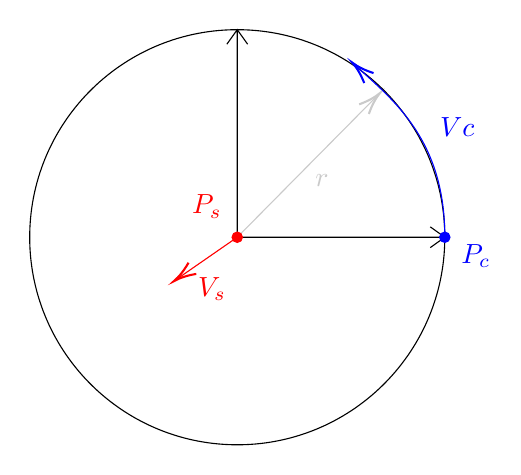
\begin{tikzpicture}[x=0.75pt,y=0.75pt,yscale=-1,xscale=1]
%uncomment if require: \path (0,300); %set diagram left start at 0, and has height of 300

%Straight Lines [id:da5485055431259082] 
\draw [color={rgb, 255:red, 202; green, 202; blue, 202 }  ,draw opacity=1 ]   (350,150) -- (417.35,81.94) ;
\draw [shift={(418.76,80.52)}, rotate = 134.7] [color={rgb, 255:red, 202; green, 202; blue, 202 }  ,draw opacity=1 ][line width=0.75]    (10.93,-3.29) .. controls (6.95,-1.4) and (3.31,-0.3) .. (0,0) .. controls (3.31,0.3) and (6.95,1.4) .. (10.93,3.29)   ;
%Shape: Circle [id:dp6398912459751643] 
\draw   (250.01,148.71) .. controls (250.72,93.48) and (296.07,49.3) .. (351.29,50.01) .. controls (406.52,50.72) and (450.7,96.07) .. (449.99,151.29) .. controls (449.28,206.52) and (403.93,250.7) .. (348.71,249.99) .. controls (293.48,249.28) and (249.3,203.93) .. (250.01,148.71) -- cycle ;
%Shape: Axis 2D [id:dp3647393603318628] 
\draw [color={rgb, 255:red, 0; green, 0; blue, 0 }  ,draw opacity=1 ] (350,150) -- (450,150)(350,50) -- (350,150) -- cycle (443,145) -- (450,150) -- (443,155) (345,57) -- (350,50) -- (355,57)  ;
%Shape: Circle [id:dp47105004014911167] 
\draw  [color={rgb, 255:red, 255; green, 0; blue, 0 }  ,draw opacity=1 ][fill={rgb, 255:red, 255; green, 0; blue, 0 }  ,fill opacity=1 ] (347.5,150) .. controls (347.5,148.62) and (348.62,147.5) .. (350,147.5) .. controls (351.38,147.5) and (352.5,148.62) .. (352.5,150) .. controls (352.5,151.38) and (351.38,152.5) .. (350,152.5) .. controls (348.62,152.5) and (347.5,151.38) .. (347.5,150) -- cycle ;
%Shape: Circle [id:dp5004065866817864] 
\draw  [color={rgb, 255:red, 0; green, 0; blue, 255 }  ,draw opacity=1 ][fill={rgb, 255:red, 0; green, 0; blue, 255 }  ,fill opacity=1 ] (447.5,150) .. controls (447.5,148.62) and (448.62,147.5) .. (450,147.5) .. controls (451.38,147.5) and (452.5,148.62) .. (452.5,150) .. controls (452.5,151.38) and (451.38,152.5) .. (450,152.5) .. controls (448.62,152.5) and (447.5,151.38) .. (447.5,150) -- cycle ;
%Straight Lines [id:da22346520312248852] 
\draw [color={rgb, 255:red, 255; green, 0; blue, 0 }  ,draw opacity=1 ]   (350,150) -- (321.07,170.05) ;
\draw [shift={(319.42,171.19)}, rotate = 325.28] [color={rgb, 255:red, 255; green, 0; blue, 0 }  ,draw opacity=1 ][line width=0.75]    (10.93,-3.29) .. controls (6.95,-1.4) and (3.31,-0.3) .. (0,0) .. controls (3.31,0.3) and (6.95,1.4) .. (10.93,3.29)   ;
%Curve Lines [id:da013980587438244485] 
\draw [color={rgb, 255:red, 0; green, 0; blue, 255 }  ,draw opacity=1 ]   (450,150) .. controls (450.09,103.06) and (425.37,84.14) .. (406.84,67.16) ;
\draw [shift={(405.42,65.86)}, rotate = 42.88] [color={rgb, 255:red, 0; green, 0; blue, 255 }  ,draw opacity=1 ][line width=0.75]    (10.93,-3.29) .. controls (6.95,-1.4) and (3.31,-0.3) .. (0,0) .. controls (3.31,0.3) and (6.95,1.4) .. (10.93,3.29)   ;

% Text Node
\draw (327,128.4) node [anchor=north west][inner sep=0.75pt]  [color={rgb, 255:red, 255; green, 0; blue, 0 }  ,opacity=1 ]  {$P_{s}$};
% Text Node
\draw (456.67,152.07) node [anchor=north west][inner sep=0.75pt]  [color={rgb, 255:red, 0; green, 0; blue, 255 }  ,opacity=1 ]  {$P_{c}$};
% Text Node
\draw (329.83,168.29) node [anchor=north west][inner sep=0.75pt]  [color={rgb, 255:red, 255; green, 0; blue, 0 }  ,opacity=1 ]  {$V_{s}$};
% Text Node
\draw (446.5,90.96) node [anchor=north west][inner sep=0.75pt]  [color={rgb, 255:red, 0; green, 0; blue, 255 }  ,opacity=1 ]  {$Vc$};
% Text Node
\draw (386.38,118.66) node [anchor=north west][inner sep=0.75pt]  [color={rgb, 255:red, 202; green, 202; blue, 202 }  ,opacity=1 ]  {$r$};

\draw [draw opacity=0]  (448.43,145.96) -- (451.51,149.04)(451.51,145.96) -- (448.43,149.04) ;
\draw [draw opacity=0]  (448.43,150.96) -- (451.51,154.04)(451.51,150.96) -- (448.43,154.04) ;
\draw [draw opacity=0]  (448.46,148.36) -- (451.54,151.44)(451.54,148.36) -- (448.46,151.44) ;
\draw [draw opacity=0]  (429.08,89.28) -- (432.16,92.36)(432.16,89.28) -- (429.08,92.36) ;
\draw [draw opacity=0]  (408.2,68.26) -- (411.28,71.33)(411.28,68.26) -- (408.2,71.33) ;
\end{tikzpicture}
\end{center}
\end{minipage}

The restatement of this problem also prompts restating the question: \textit{What path does it trace?}

We will assume both animals to be acting \textit{nearly optimally}, so are choosing whichever option gives them the best result in the moment, or when two or more solutions are equally optimal we will make sure to define one of them to always be picked to avoid ambiguity. In Cat's case it is trying to be closer to the Swan, since its "win condition" is essentially having the same position as the Swan on the lake border. It is also required that they can observe the behaviour of the other animal and make decisions based on that, so all the information is open. In game theory this is often called "deterministic"\textcolor{red}{CITE} games, since all participating parties have perfect\textcolor{red}{CITE} information.

When solving this problem it is useful to think in terms of strategies like one would in game theory. This mental model yield a perspective of two competing actors trying to optimize for criteria which expedites insight. 

\section{Solution}

The Cat has the simplest win condition out of all that can be satisfied, so it makes sense to look at it first. Since it has to have 0 distance to the Swan we can think of it as trying to minimize it's position in relation to the Swan. One way to minimize the distance is to move towards the Swan at all times and this way proves itself most effective:

\textbf{Theorem}: The best strategy for the Cat to act is to always move closer to the Swan.

\textbf{Proof}:
\begin{enumerate}
	\item Let point $p$ be a projection of the Swan's velocity $V$ on the circle.
	\item Let the Cat be moving towards some point $p^\dagger$ on the circle shore.
	\item If $p = p^\dagger$ then the Cat catches the Swan and the Cat wins. 
	\item In case that $p \neq p^\dagger$, let there be some arc $C$ along the circle traced from the position of the Cat to it's desired destination $p^\dagger$.
	\item If $p$ does not belong to said arc $C$ the Swan wins.
	\item In case that $p \in C$, the Swan can direct its velocity at $-V$, which will correspond to a point $-p$ that is not on the arc $C$. $\blacksquare$
t\end{enumerate}

The same logic, sadly, does not express the variety of the Swan's potential strategies, since it's goal is not to actually get away from the Cat, but to reach the shore without being caught. One of the first things you can do when approaching such question is look at whether it even is solvable.

\subsection{The Dash Distance}

The first question that anyone looking at this problem comes up is: ``well, can't the Swan just swin to the shore?''. Yes, the simplest strategy for the Swan is to swim towards the shore in a straight line without ever changing direction, it is the shortest path after all (by definition of what a line is\textcolor{red}{CITE} anyway). We will denote the velocities of the Swan and the Cat as $V$ and $V'$ respectively. The time $t$ it takes the Swan to reach the shore will be $\frac{r}{V}$. In Cat's case it entirely depends on the point, for example to reach the point opposite to it's current is going to take $t' = \frac{\pi r}{V'} = \frac{\pi r}{4V}$. Notice that even if the Swan swims directly away from the Cat's initial position it will be caught:

\textbf{Theorem:} The Cat will outrun the Swan if the Swan swims directly opposite to the Cat's initial position.

\textbf{Proof:} Assume 
\begin{center}
$\begin{WithArrows}
\text{t} &< \text{t'} \Arrow{Substitute}\\
\frac{\pi r}{V'} &< \frac{r}{V} \Arrow{$V' = 4V$}\\
\frac{\pi r}{4V} &< \frac{r}{V} \Arrow{$\square \cdot \frac{V}{r}$}\\
\frac{\pi}{4} &< 1 \hspace{10pt} \blacksquare
\end{WithArrows}$
\end{center}

We see that the just dashing to the edge won't work for the Swan if it's in the middle, but we can imagine alternative conditions. If the Swan is closer to the edge, surely it could be faster than the Cat?

Assume the Swan is such distance $d$ away from edge and directly opposite the Cat, so that it can safely reach the edge. That would mean that the time it takes the Swan to reach the edge is shorter, than the time it takes the Cat to reach the same point. It of course depends on the position of the Cat, but let it be exactly opposite the Swan. It can be expressed as $\frac{d}{V} < \frac{\pi r}{4V} \Leftrightarrow  d < \frac{\pi}{4}r$.

\subsection{The Freedom Circle}

Now the question is whether it is even possible to get to that point. We can turn our attention to the angular velocities of the animals, since both of them are moving around the circle. If the distance of the Swan from the center is $D = r - d$, the Swan has the angular velocity of $\omega = \frac{V}{D}$ and the Cat has angular velocity $\omega' = \frac{4V}{r}$. Notice how the velocity of the Cat is essentially constant, but the velocity of the Swan is controlled by its distance from the center $D$. Based on this we can solve for $D$, at which the Swan is angularly faster than the Cat.

\begin{center}
$\begin{WithArrows}[jot=2ex]
\frac{V}{D} &> \frac{4V}{r} \Arrow{$\square^{-1}$}\\
\frac{D}{V} &< \frac{r}{4V} \Arrow{$\square \cdot {V}$}\\
D &< \frac{r}{4} \Arrow{$D = r - d$}\\
r - d &< \frac{r}{4} \Arrow{$\square - r$}\\
- d &< \frac{r}{4} - r  \Arrow{$\square \cdot (-1)$}\\
d &> \frac{3}{4}r
\end{WithArrows}$
\end{center}

So far all points that are $D$ or less away from the center (inside the ``freedom'' circle of radius $D$)the Swan is faster, based on that I claim it can occupy any position inside, positioning itself anywhere relative to the Cat.

Notice that there can exist such $d$ that $r - \frac{r}{4} < d < \frac{\pi}{4}r$. Given that $r = 1$ we get to know that the distance of the Swan from the edge has to be $\frac{3}{4} < d < \frac{3.14\dots}{4}$.
The set of all points inside the circle that are $d$ away forms an annulus, such that when the Swan is inside this annulus and the Cat is opposite the Swan, it may dash to the edge of the lake and flee, so the trajectory must exist.

\textbf{Theorem}: There exists an infinite amount of viable trajectories.

\textbf{Proof}: For every possible trajectory, the Swan can make a lap inside the ``freedom'' circle one more time, giving us a new trajectory. 

\subsection{Describing Velocity}

Next we may look at getting to the edge of the "safety" annulus. For a successful escape the Swan has to exit it at such point, that it's directly opposite the Cat. Over an infinitesimal amount of time $\Delta t$ the Swan can travel a total distance of $s = V \Delta t$. Assume the Swan is somewhere inside the ``freedom'' circle, then the Cat moves at $\omega' = \pm \frac{4V}{r}$. The Cat can move either clockwise or counterclockwise, since at all times there are two paths to its desired point and the Cat is always going to choose the shortest (except for the case when cat is directly opposite, since then two paths have equal lengths, when that happens we will assume the cat to move counterclockwise $\omega' > 0$).

In this case in order to compensate for the Cat's movement (remain opposite to it) the Swan has to move the same angle in \textit{the same direction around the clock, but opposite in terms of coordinates}. Since the magnitude of the velocity vector should remain $V$, we can express it as two vectors: moving away from the center to exit the ``freedom'' circle ($V_\alpha$) and compensation for Cat's movement ($V_{\omega'}$). If compensation is $V_{\omega'} = \omega' \cdot D$, we can solve for the away velocity ($V_\alpha$) as follows:

\begin{center}
$\begin{WithArrows}[jot=2ex]
V &= \sqrt{(\omega'D)^2  + V_\alpha^2} \Arrow{$\square^2$}\\
V^2 &= (\omega'D)^2  + V_\alpha^2 \Arrow{$\square - (\omega'D)^2$}\\
V_\alpha^2 &= V^2 - (\omega'D)^2 \Arrow{$\sqrt{\square}$}\\
V_\alpha &= \pm\sqrt{V^2 - (\omega'D)^ 2}
\end{WithArrows}$
\end{center}

We can ignore the possible negative values of $V_\alpha$, since the magnitude of the velocity vector can never be negative. Based on that I conclude that $V_\alpha = \sqrt{V^2 - (\omega' D)^2}$.

\begin{center}
	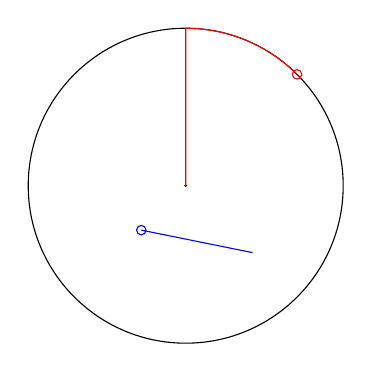
\begin{tikzpicture}[scale=2]
		\draw (0,0) circle [radius=1];
		\fill[color=black] (0,0) circle [radius=0.01];
		\draw[color=red] (0.707,0.707) circle [radius=0.03];
		\draw[color=blue] (-0.282,-0.282) circle [radius=0.03];
		\draw[color=red] (0.707,0.707) 
		arc[start angle = 45, end angle = 90, radius=1]
		(0, 0) -- (0, 1);
		\draw[color=blue] (-0.282, -0.282) -- (0.425, -0.425);
		
	\end{tikzpicture}
\end{center}

When describing the motion of objects in a 2D plane like in our case it only makes sense to use vectors, however, since we often deal with angles an rotations a polar complex coordinate system is a lot more appropriate. We will define $i$ such that $i = \sqrtsign{-1}$ and assume 1 and $i$ to be the vector bases for $\{z \in \mathbb{C}: z = 1x + iy\}$.

We can introduce a polar coordinate system to get the velocities for the Swan or the Cat as complex numbers $\vec{V}$ and $\vec{V}'$ respectively. Since the Cat always moves tangentially, let $\theta$, the angle between the Cat's position and the x-axis, then its velocity will always be directed at angle $\theta \pm \pi$ relative to the x-axis (tangentially to the circle, counterclockwise or clockwise depending on the $\pm \pi$).

To get the angle we can imagine the complex number to be describing a line, since the real part is usually considered the x coordinate and the imaginary is the y, the slope of the line going through that point is $\frac{y}{x}$, so for $1x + iy$ it is $\tan \theta = \frac{y}{x}$, so to get the angle we apply $\arctan$ to both sides, that yields $\theta = \arctan{\frac{y}{x}}$, the definition of the \textit{principal argument}\cite{princarg} or the \textit{phase} of a complex number denoted $\arg z$. There is an issue with purely imaginary numbers (when there is no real component, $\Re (z) = 0$), since in that case $\arg$ would be undefined. To avoid this issue we may extend this function to the following: $$
\arg (z) = \left\{ 
		\begin{aligned}
			\pi						,\hspace{4pt}&  z = 0 + |z|i\\
			-\pi					,\hspace{4pt}&  z = 0 - |z|i\\
			\arctan {\frac{\Im (z)}{\Re (z)}}	,\hspace{4pt}&	\text{otherwise}\\
		\end{aligned}
	\right.$$

To decide whether to move clockwise or counterclockwise the Cat can use the cross product of its own and the Swan's positions $P_s \times P_c$, specifically the imaginary component. Due to the properties of the cross product it will always yield a vector perpendicular to the initial two, but since we are restricted to be inside a complex plane, the only vector component is imaginary. Given that complex numbers are vectors with bases $1$ and $i$, the cross product is just the determinant of a joined matrix of vectors: $P_s \times P_c = \det \bigl[ \begin{smallmatrix} 
	a & c\\
	ib & id 
  \end{smallmatrix} \bigr] = iad - ibc = i(ad - bc)$.

From that we see that the only vector component is, indeed, imaginary, so we define $p_\times = \Im{(P_cs \times P_c)}$ and verify that it's sign will match the optimal direction (clockwise or counterclockwise):

\textbf{Theorem}: Cross product of two vectors is negative when going clockwise is fastest and negative is counterclockwise is faster.

\textbf{Proof}: 
Let there be $x = a + ib$, $y = c + id$ and $\Delta = x \times y$. We can reason from the perspective of $y$ by performing a proper rotation\cite{rotation} of both vectors by $y$. Their orientations remain the same, so the cross product has to be is preserved. This rotation will transform $x$ into $\frac{x}{y} = \frac{a + ib}{c + id}$ and $y$ into $\frac{y}{y} = 1 + 0i$. By its geometric definition $\Delta = |x| |y| \sin (x \angle y)$. 

After the transformation, $x \angle y$ is the angle between $x$ and the x-axis, so it is $\arg x$ by definition, giving $\Delta = |\frac{a + ib}{c + id}| |1 + 0i| \sin (\arg x)$. Magnitudes of $x$ and $y$ always yield non-negative values, so the only term that changes the sign is sine. $\sin (\arg x)$ is positive for $\arg x \in (0; \pi)$, so when $x$ is in the upper semicircle and is negative when $\arg x \in (\pi; 2\pi)$ when $x$ is in the lower semicircle.

The clockwise angular distance to a point on the upper semicircle is $s_{\text{cw}} = \arg x$ and the counterclockwise distance is $s_\text{ccw} = \pi - \arg x$. If $\arg x \in (0; \pi)$ then $s_\text{cw} < s_\text{ccw}$ and $\Delta > 0$, else if $\arg x \in (\pi; 2\pi)$ then $s_{\text{ccw}} < s_{\text{cw}}$ and $\Delta < 0$. $\blacksquare$

One of the problems that may also arise is that the cross product of two collinear\cite{vectorterminology} vectors is $0$, in our case that would happen when the Swan is either moving directly at the Cat or directly away. However, since we defined the Swan's strategy to require always moving in the opposite direction, we can omit the case of the vectors being collinear and parallel\cite{vectorterminology} and only focues the collinear and antiparallel\cite{vectorterminology} case.

Since scaling the cross product would also influence the magnitude of the velocity vector we will use the signum function. $$\text{sgn}(x) = \left\{ 
	\begin{aligned}
		-1&, x < 0\\
		0&, x = 0\\
		1&, x > 0
	\end{aligned}
\right.$$

The main issue with this classic definition is that it is $0$ at $x = 0$, in our problem domain this would correspond to the Cat getting stuck when it is opposite the Swan, for that purpose we will define another function, to insist going counterclockwise in an ambigous case:$$\text{sgn}_+(x) = \left\{ 
	\begin{aligned}
		-1&, x < 0\\
		1&, x \geq 0
	\end{aligned}
\right.$$

Combining insight given by everything above, the final equation for describing the Cat's motion is $$
\vec{V}' = 4 \cdot \text{ sgn}_+ (p_\times) \cdot e^{i (\theta + \frac{\pi}{2})}
$$

4 comes from the fact that the Cat's speed is four times that of the swan, $\text{sgn}_+$ ``decides" the Cat's direction (clockwise or counterclockwise) and $e^{i (\theta + \frac{\pi}{2})}$ is a complex vector, directed tangentially to the circle, with $\theta$ being the $\arg P_cs$. 

The Swan on the other hand will have to decide on the strategy depending on the distance $D$ from the center. When dashing away its velocity vector will be directed away from the center, exactly where the magnitude of its position $P_cs$ is directed.

\begin{equation*}
	\vec{V} = \left\{ 
		\begin{aligned}
			\frac{\vec{V}'}{4} (i V_\alpha  - \omega' D) & \text{,   inside ``freedom'' circle} \\
			\frac{P_s}{|P_s|} & \text{,   opposite the Cat in the ``safety'' annulus}
		\end{aligned}
	\right.
\end{equation*}

We had to use a clever $\text{sgn}$ function to describe the direction, however, when looking at the simulated behaviour of a Cat, one thing becomes apparent: at no point does it have to turn around.

\textbf{Theorem}: Cat will always be moving in the same direction.

\textbf{Proof}: Let's assume without any loss of geneality the Cat and the Swan are moving step by step starting with the initial conditions. Then either the Cat or the Swan has to start moving first. 
For the Cat never to turn around it has to have prefer motion in a consistent direction in four cases: in the very beginning (case A), when the Swan is ``dashing'' to the edge (case B) and when the Swan is in the ``freedom'' circle (case C).

\textbf{A}: Let the Cat move first. We defined it to move counterclockwise in ambigous conditions, so that's what it will do. Since the Swan is at origin, the Cat will move counterclockwise (as defined by $\text{sgn}_+$). This only changes the specific position $P_c$, whereas its position relative the Swan stays the same, therefore the conditions are identical to initial so the direction is \textit{counterclockwise}.

Let the Swan move first, it will prefer going directly away from the Cat. That would still position it directly opposite, so the Cat would prefer going \textit{counterclockwise}.

\textbf{B}: By definition the swan starts ``dashing'', when it is exactly opposite the Cat, that implies that the Cat has the same distance to whatever shore point corresponds to Swan's current position. In ambigous cases the Cat prefers going \textit{counterclockwise}.

\textbf{C}: For every angular displacement of the Cat, the same angular displacement is replicated by the Swan in the same direction around the clock by definition of $\vec{V}'$, so if the Cat starts moving \textit{counterclockwise} (see A) the Swan will follow in the same direction.

In all of the above cases the will move \textit{counterclockwise}. Beyond that, if the initial conditions defined the Cat to move \textit{clockwise} in an ambigous case, all the other cases would follow, so there is nothing special about the direction. $\blacksquare$.

The proof above allows us to redefine $V' = 4 \cdot e^{i (\theta + \frac{\pi}{2})}$ and can simplify the equation of motion for the Swan in the ``freedom'' circle:

\begin{center}
	$\begin{WithArrows}[jot=2ex]
		\vec{V} &= \frac{\vec{V}'}{4} (i V_\alpha  - \omega' D) \Arrow{Substitute V'} \\
		&= \frac{4 \cdot e^{i (\theta + \frac{\pi}{2})}}{4} (i V_\alpha  - \omega' D) \Arrow{Simplify the constant}\\
		&= e^{i (\theta + \frac{\pi}{2})} (i V_\alpha  - \omega' D) \Arrow{Simplify $e^{i\frac{\pi}{2}}$}\\
		&= e^{i\theta} i (i V_\alpha  - \omega' D) \Arrow{Multiply i into the parentheses}\\
		&= e^{i\theta} \cdot (-V_\alpha + i\omega'D) \Arrow{Substitute $V_\alpha$}\\
		&= e^{i\theta} (-\sqrt{V^2 - (\omega' D)^2} + i\omega'D) \Arrow{Distribute $e^{i\theta}$}\\
		&= -e^{i\theta} \sqrt{V^2 - (\omega' D)^2} + ie^{i\theta}\omega'D
	\end{WithArrows}$
\end{center}

Based on this we can entirely exclude $\text{sgn}_+$ from the equation, which simplifies it a lot. This equation for motion only depends on $D$ (the distance from the center) and $\omega'$ (the angular compensation), all the other letters denote constants, so $V(D, \omega')$.

giving the final two equations for motion of both animals:


\begin{multicols}{3}
	\begin{equation*}
		\vec{V} = \left\{ 
			\begin{aligned}
				-e^{i\theta} \sqrt{V^2 - (\omega' D)^2} + ie^{i\theta}\omega'D \\
				\frac{P_s}{|P_s|} &, \theta = 0
			\end{aligned}
		\right.
	\end{equation*}
\end{multicols}


\subsection{Changing The Reference Frame}

At this point the problem is essentially solved, the trajectory is found but the discovered result is not very interesting not very intuitive. The last step in this problem is to change the reference frame. We can ``pin'' the Cat in place and let the Lake spin on its own, favouring the Cat. In this case the spin of the rotating Lake is the Cat's angular velocity $\omega'$.

This idea came to me when studying circular motion in the physics class. This allows us to characterize the Space as a vector field defined by $f: \mathbb{R}^2 \rightarrow \mathbb{R}^2$ or in our case $\vec{V}: (\mathbb{R}_{[0; 2\pi[}, \mathbb{R}^+) \rightarrow \mathbb{C}$, where $V(\theta, D)$. This interpretation furthers the intuition, since it associates every possible state of the Swan with a corresponding velocity.

Furthermore, since $D$ is a non-negative value and $\theta$ is the angle their combination produced a complex number $z = De^{i\theta}$ which is equal to the Swan's position at the circle if the Cat is fixed, so in this context $P_s = De^{i\theta}$. To avoid confusion we may denote this new function $\nu(P_s)$, which gives the velocity of the Swan on a fixed circle given a fixed position. However, it would be much more useful to look at the position instead of the instant velocity. For that we may integrate the velocity:

\begin{center}
	$\begin{WithArrows}[jot=2ex]
		\vec{V} &= -e^{i\theta} \sqrt{V^2 - (\omega' D)^2} + ie^{i\theta}\omega'D \Arrow{Expand $(\omega' D)^2$}\\
		&= -e^{i\theta} \sqrt{V^2 - \omega'^2 D^2} + ie^{i\theta}\omega'D \Arrow{Substitute D}\\
		&= -e^{i\theta} \sqrt{V^2 - \omega'^2 ((\Im D)^2 + (\Re D)^2)} + ie^{i\theta}\omega'D
	\end{WithArrows}$
\end{center}

\section{Evaluation}

\section{Conclusion}

The solution to the problem might have not been the most insightful in history of sciences, there isn't a field based on this formula nor is it vital to the existance of our human society. I found the journey of exploring this problem very enjoyable and got to apply my newly gained skill. Over the course of working on this project I  looked into many fields which I did not find useful to mention (numerical analysis, geometric algebra)

\section*{Appendix}

\begin{tabular}{|l|l|}
\hline
\textbf{Variable} & \textbf{Purpose}\\
\hline
$r \in {\mathbb{R}^+}$ & The radius of the lake\\
$d \in \{x \in \mathbb{R^+}: 0 \leq x < r \}$ & Distance of the Swan from the edge\\
$D = r - d$ & Distance of the Swan from the center, magnitude of position\\
$V \in {\mathbb{R}^+}$ & Magnitude of the Swan's velocity\\
$V' = 4V$ & Magnitude of the Cat's velocity\\
$\vec{V}' \in \mathbb{C}$ & Complex velocity vector of the Cat\\
$\vec{V} \in \mathbb{C}$ & Complex velocity vector of the Swan\\
$\omega \in \mathbb{R}_{2\pi}$ & The angular velocity of the Swan\\
$\omega' \in \mathbb{R}_{2\pi}$ & The angular velocity of the Cat\\
$V_{\omega'} \in \mathbb{R^+}$ & Swan's linear compensation for Cat's angular velocity\\
$V_\alpha \in \mathbb{R^+}$ & Swan's velocity component directed away from the Cat\\
$P_s \in \mathbb{C}$ & Position of the Swan\\
$P_c \in \mathbb{C}$ & Position of the Cat\\
$\theta$ & Angular distance of the Cat from the x-axis\\
$p_\times$ & Cross product of the Cat's and Swan's positions\\
\hline
\end{tabular}
\vspace{12pt}

\bibliographystyle{plain}
\bibliography{sources}
\end{document}
